\newpage
\section*{Exercise 1 (comments by Sen)}
The following code defines a function, called LCG to generate random numbers between 0 and 1 given multiplier a, shift c, modulus M, $x_0$ and size.

\begin{python}
# x_i = mod (a * x_(i-1) + c, M);  U_i = x_i / M

def LCG(a, c, M, x_0, size):
    LCG_set = [0] * size
    LCG_set[0] = (x_0 * a + c) % M
    
    for i in range(1, size):
        LCG_set[i] = (LCG_set[i-1] * a + c) % M
        
    return [entry / M for entry in LCG_set] 
\end{python}

The results are shown in figure \ref{fig:lcgHist} and figure \ref{fig:lcgScat}, indicating that the random numbers from LCG are not uniformly distributed and are indeed correlated.

\begin{figure}[h]
\centering
\begin{minipage}{.5\textwidth}
  \centering
  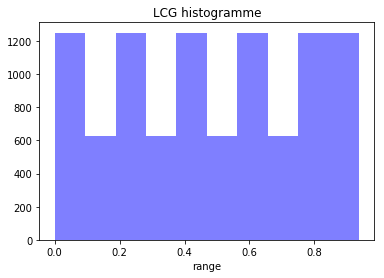
\includegraphics[width=0.95\linewidth, height = 0.75\linewidth]{figures/lcgHist.png}
  \caption{Histogramme of LCG}
    \label{fig:lcgHist}
\end{minipage}%
\begin{minipage}{.5\textwidth}
  \centering
  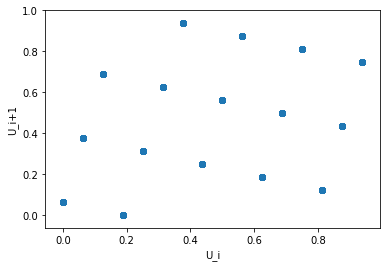
\includegraphics[width=0.95\linewidth, height = 0.75\linewidth]{figures/lcgScat.png}
  \caption{Scattering plot of LCG}
  \label{fig:lcgScat}
\end{minipage}
\end{figure}


Statistical tests including $\chi^2$, KS, run test and correlation test are performed and covered in the following part.

\subsection*{$\chi^2$ test}
The $\chi^2$ test is performed as follows. The test statistic T is equal to 937.5, which is much high than the critical value of 3.32 at a confidence level of 95\%, indicating that the LCG generated numbers are not uniformly distributed. 
\begin{python}
# chi square test
def chisquared(setA, setB):
    nclass = len(setA)
    T = sum([(setB[i]-setA[i])**2/setA[i] for i\
             in range(nclass)])
    return T
def count(set, min, max):
    n = 0
    for i in set:
        if (min <= i) and (i < max):
            n += 1
    return n  

expe = [1000] * 10
real = [0] * 10
for i in range(10):
    real[i] =  count(set1, 0.1*i, 0.1 * i+ 0.1)    
print(chisquared(expe, real))
\end{python}

\subsection*{Kolmogorov Smirnov test (KS test)}
The following code defines a function called kstest that can be used to calculated the test statistic $D_n$ for comparison with uniform distribution. 
\begin{python}
# KS test, only for comparison with uniform distribution
def kstest(setA):
    set_sorted = sorted(setA)
    sup = [0] * len(setA)
    for i in range(len(setA)):
        sup[i] = abs(1/len(setA) * (i+1) - set1_sorted[i])
    Dn = max(sup)
    return Dn
    
Dn = kstest(set1)
\end{python}
In our case, the statistic is 0.0625. The adjusted statistic is 6.26 using the following definition: $\left(\sqrt{n}+0.12+\frac{0.11}{\sqrt{n}}\right) D_{n}$, which is a lot larger than 1.628, so we have a confidence level of 99.0\% to reject the null hypothesis (i.e. we reject that the LCG generated numbers are uniformly distributed).

\subsection*{Run test I}
For run test I, numbers of above the median and below are computed. Using these, the mean and variance of the normal distribution can be calculated. Then the following variable should have a standard normal distribution:
\begin{equation}
    \frac{N_{run} - \mu} {\sigma} \sim N(0,1)
\end{equation}
The calculated result is -25, which indicates that the LCG generated random numbers are indeed correlated.
\begin{python}
# run test 1
import statistics as stt
import math
def runTest1(setA):
    median1= stt.median(setA)
    up = 0
    down = 0
    for i in setA:
        if i <= median1:
            down += 1
        else:
            up += 1
    run = 1
    for i in range(len(setA)-1):
        if (setA[i]<= median1 and setA[i+1] >median1) or\
        (setA[i]>median1 and setA[i+1] <=median1):
            run += 1
    mu = 2 * up * down / (up + down) + 1
    sigma = math.sqrt((2*up*down * (2*up*down-up-down))/\
                      ((up + down)**2 * (up + down-1)))
    return (run - mu) / sigma
\end{python}
\subsection*{Run test II}
The following code defines a runTest2 function, returning the test statistic. The result for the LCG generator is 1118.8, which is way bigger than the critical value, examining that the LCG generated random numbers are indeed correlated.
\begin{python}
from numpy import *
def runTest2(setA):
    A = mat([[4529.4, 9044.9, 13568, 18091, 22615, 27892],\
             [9044.9,18097, 27139, 36187, 45234, 55789],\
             [13568, 27139, 40721, 54281, 67852, 83685],\
             [18091, 36187, 54281, 72414, 90470, 111580], \
             [22615, 45234, 67852, 90470, 113262, 139476], \
             [27892, 55789, 83685, 111580, 139476, 172860]])
    B = mat([1/6, 5/24, 11/120, 19/720, 29/5040, 1/840])
    index = [0]
    for i in [ind+1 for ind in range(len(setA)-1)]:
        if setA[i] < setA[i-1]:
            index.append(i)
    index.append(len(setA))  
    
    orderSet = [index[i+1]-index[i] for i in range(len(index)-1)]
    R = [0] * 6
    for i in orderSet:
        if i == 1:
            R[0] += 1
        elif i == 2:
            R[1] += 1
        elif i == 3:
            R[2] += 1
        elif i == 4:
            R[3] += 1
        elif i == 5:
            R[4] += 1
        else:
            R[5] += 1
    R = mat(R)
    Z = 1/(len(setA)-6) * (R - len(setA)* B) * \
    A *(R.T - len(setA)* B.T)
    return Z
\end{python}
\subsection*{Correlation test}
In the correlation test, 100 tests are performed with different h value from 1 to 100. Then 100 $c_h$ values are generated, which should have a normal distribution of N(0.25, $\frac{7}{144n}$) with n = 10,000. In order to test if the generated $c_h$ values satisfy the aforementioned distribution, a $\chi^2$ is done with 10 intervals from -5$\sigma$ to 5 $\sigma$. The obtained statistic T is 9887, indicating the data are correlated.
\begin{python}
# correlation
import scipy.stats as stats
def count1(x, set):
    num = 0
    for j in set:
        if x <=j and j < x+1:
            num += 1
    return num
def corre(setA):
    test = 100
    n = len(setA)
    c = [0] * test
    for h in range(test):
        h1 = h + 1
        c[h] = 1/(n-h1)* sum ([setA[i]*setA[i+h1] \
                               for i in range(n-h1)])  
    c1 = [(c[i]-0.25)/(math.sqrt(7/144/n)) for i in range(test)]   
    # chi square test for 10 intervals from -5sigma to 5 sigma
    expected = [n*(stats.norm.cdf(-4 + i)-stats.norm.cdf(-5 + i)) \
                for i in range(10)]
    observed = [count1(i-5, c1) for i in range(10)]
    return chisquared(expected, observed)
print(corre(set2))
\end{python}

As a comparison, random function from Numpy package, Python are visually shown and tested as well. Obviously, the generated results are more even and not related. See table \ref{tab:lcg} for detailed information. It is noteworthy that in the correlation test, the $c_h$ values are close to 0.25, but the variance is much higher than $\frac{7}{114n}$, which explains why the T statistic is also high for the standard generator.
\begin{figure}[h]
\centering
\begin{minipage}{.5\textwidth}
  \centering
  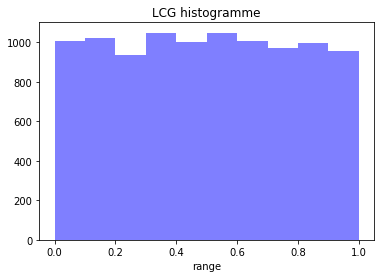
\includegraphics[width=0.95\linewidth, height = 0.75\linewidth]{figures/numpyHist.png}
  \caption{Histogramme of numpy}
    \label{fig:numpyHist}
\end{minipage}%
\begin{minipage}{.5\textwidth}
  \centering
  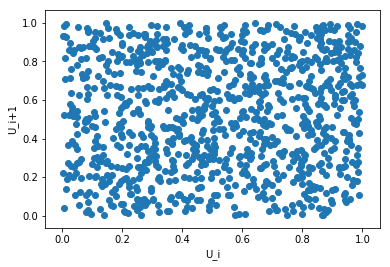
\includegraphics[width=0.95\linewidth, height = 0.75\linewidth]{figures/numpyScat.png}
  \caption{Scattering plot of numpy}
  \label{fig:numpyScat}
\end{minipage}
\end{figure}

\begin{table}[h]
    \centering
    \begin{tabular}{|c|c|c|c|}
    \hline
      Test  & Parameter &  LCG & Standard\\
    \hline
    $\chi^2$ test & T & 937.5 & 11.7 \\ \hline
    KS test & $D_n$ & 0.0625 & 0.0106 \\ \hline
    Run test I & $\frac{N_{run}-\mu}{\sigma}$& -25.00 &0.02\\ \hline
     Run test II   &Z & 1118.8  & 3.5968 \\ \hline
     Correlation test & T& 9887 &9805 \\ \hline
    \end{tabular}
    \caption{Tested result of LCG and standard built-in random number generator}
    \label{tab:lcg}
\end{table}